% ICRC-2021 
% Deadline 5 July
% Maximum 8 pages

% Please make sure you insert your
% data according to the instructions in PoSauthmanual.pdf
\documentclass[a4paper,11pt]{article}
\usepackage{pos} 

\usepackage[utf8]{inputenc} % Включаем поддержку UTF8
\usepackage[T2A]{fontenc}
\usepackage[russian,english]{babel}   % убрать русский перед отправкой статьи % влияет на язык подписей к рисункам и таблицам
\usepackage[modulo]{lineno}
\usepackage{graphicx}
\graphicspath{{figures/}}
%\usepackage[pdftex, backref, colorlinks]{hyperref}
\usepackage{todonotes}
%http://ctan.math.washington.edu/tex-archive/macros/latex/contrib/easy-todo/easy-todo.pdf
%\usepackage[enable]{easy-todo}

\title{A drone-borne installation for studying the composition of cosmic rays in the range of 1--1000~PeV by registering the reflected Cherenkov light of EAS.}
\ShortTitle{SPHERE-3 project} 

%\date{June 2021}
\author*[a,b]{I. A. Vaiman}
\author[b]{D. V. Chernov}
\author[b]{E. A. Bonvech}
\author[c,d]{M. Finger}
\author[c,d]{M. Finger Jr}
\author[a,b]{V. I. Galkin}
\author[a]{V. A. Ivanov}
\author[a]{V. S. Latypova}
\author[a,b]{D. A. Podgrudkov}
\author[b]{T. M. Roganova}

\affiliation[a]{Faculty of physics, Lomonosov Moscow State University,\\Lininskie gory, 1, Moscow, Russia}
\affiliation[b]{Skobeltsyn Institute for Nuclear Physics Lomonosov Moscow State University,\\Lininskie gory, 1, Moscow, Russia}
\affiliation[c]{Faculty of Mathematics and Physics, Charles University,\\18000 Prague, Czech Republic}
\affiliation[d]{Joint Institute for Nuclear Research,\\Dubna, Russian Federation}

\emailAdd{gosha.vaiman@gmail.com}
\emailAdd{chr@dec1.sinp.msu.ru}
\emailAdd{bonvech@yandex.ru}
\emailAdd{michael.finger@cern.ch}
\emailAdd{miroslav.finger@cern.ch}
\emailAdd{v\_i\_galkin@mail.ru}
\emailAdd{ivanov.va18@physics.msu.ru}
\emailAdd{2000vi0501g@mail.ru}
\emailAdd{d.a.podgrudkov@physics.msu.ru}
\emailAdd{rogatm@yandex.ru}

\abstract{
Here we present the current technical design of the SPHERE project’s new detector. The SPHERE project is aimed at primary cosmic ray studies in the 1--1000 PeV energy range using reflected Cherenkov light. The concept of a drone-mounted detector with a photosensitive camera based on silicon photomultipliers is discussed. The combination of the reflected CL registration method with specific data analysis approaches is a unique feature of this project. The developed earlier event-by-event data analysis approach allows to carry out primary particle mass reconstruction and PCR mass composition studies with high accuracy. This is achieved through careful analysis of each EAS CL lateral distribution function without building any kind of intermediate distributions of any `typical' characteristics.
}

\FullConference{37$^{\rm{th}}$ International Cosmic Ray Conference (ICRC 2021)\\
		July 12th -- 23rd, 2021\\
		Online -- Berlin, Germany} 

%\keywords{EAS, Cherenkov light, detector, proposal}


\begin{document}

\newcommand{\todoi}[1]{\todo[inline]{ #1}}

\linenumbers
\maketitle

\listoftodos[Notes]

\tableofcontents

\section{Introduction}

Vavilov-Cherenkov radiation (or Chereknov light, CL) is produced by charge particles of an extensive air shower (EAS) in the Earth atmosphere.

The experimental technique of detecting of the reflected Vavilov--Cherenkov radiation from extensive air showers (EAS) has been known since the 70s of the last century when it was proposed by Russian academician Alexander Chudakov~\cite{chu74:VKKL74}, whose centenary is celebrated this year. 

\todoi{Написать введение. (Бонвеч)}

Ссылка на Чудакова, его 100 летие. Про метод (ЭЧАЯ).
Про проект СФЕРА. Ссылка на СФЕРУ-1. 
Помянуть "успехи" СФЕРЫ-2. Написать в духе "продолжение и развитие". (Бонвеч)

%The general idea of the SPHERE experiment is discussed: basic idea of reflected Cherenkov light registration method and it's previous implementations in the SPHERE experiment, as well as possible additions to the method that enhance its accuracy and sensitivity.

Cherenkov light, emitted when high-energy particles travel through a medium, has long been known as an important EAS registration channel. In particular, Cherenkov light lateral distribution is indicative of the shower development details and can be used to infer both the energy and the mass of the primary particle~\cite[e.g.][]{Budnev2013}.




\subsection{Reflected Cherenkov light}

The main method of Cherenkov light registration in the SPHERE project follows the idea of A. Chudakov: EAS Cherenkov light is first reflected from the <<screen>> and then observed by a detector. In previous SPHERE implementations, the snowfields of Antarctica and the snow-covered ice of Lake Baikal played the role of such screen. Snow has many desirable qualities in this regard, including a high overall albedo (up to $95\%$) and an almost isotropic bidirectional reflectance distribution \citep{Warren1982}.

To observe the reflected Cherenkov light the compact detector is lifted above the snow surface. The detector employs the Schmidt camera technique and consists of a spherical mirror with a mosaic of sensitive elements near its focal surface. In previous SPHERE implementations detectors were lifted by a balloon to an altitude of 400--1000~m with photomultipier tubes (PMT) serving as sensititve elements~\cite{Ant15a, Ant19, Ant20}. In the present paper we discuss the development of the method with a drone (UAV) as a lifting apparatus and a silicon photomultipliers (SiPM) as sensitive elements. The sketch of the technique is illustrated on Figure.~\ref{fig:DirectCL}.


\begin{figure}
    \begin{minipage}[b]{.42\textwidth}
    \centering 
        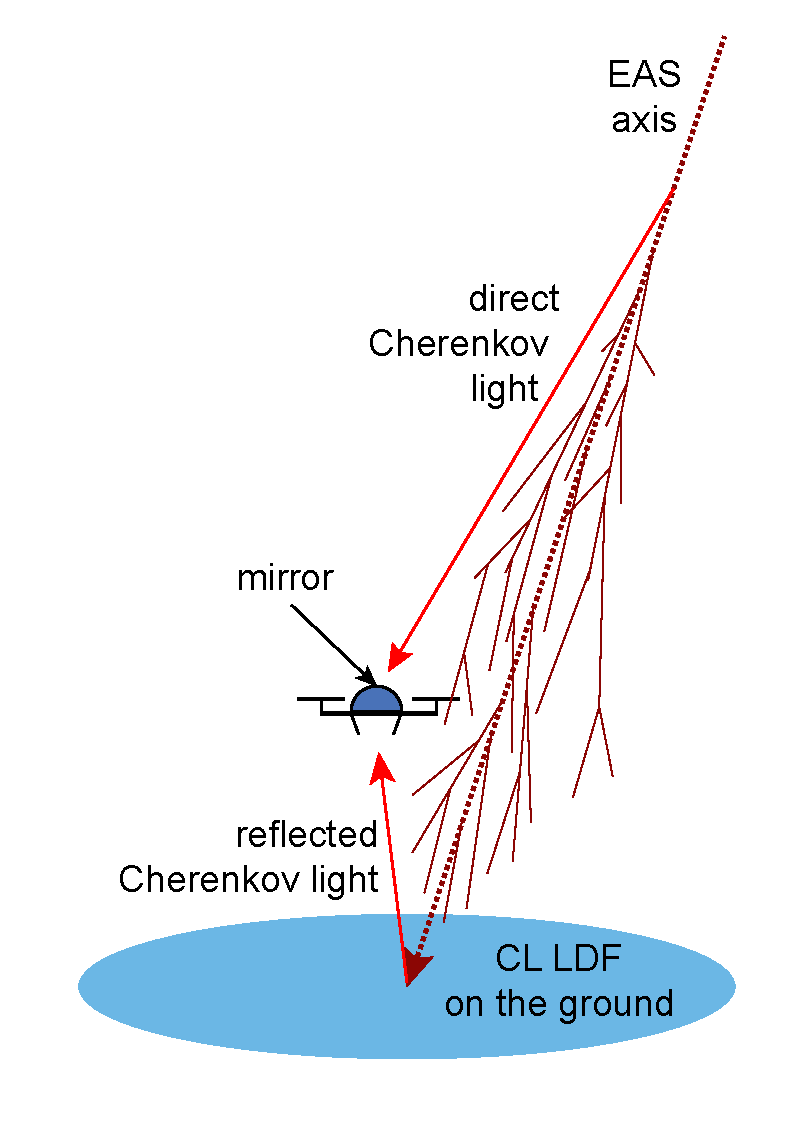
\includegraphics[height=.365\textheight]{DirectCL.pdf}
        \caption{Scheme of direct and reflected Cherenkov light from EAS.}
        \label{fig:DirectCL}
    \end{minipage}
    \hfill
    \begin{minipage}[b]{.55\textwidth}
        \centering 
        \includegraphics[height=.2\textheight, angle=0]{Sphere3optic.eps}
        \includegraphics[height=.2\textheight, angle=0]{Sphere3spot1.eps}
        \includegraphics[height=.2\textheight, angle=-90]{Sphere3spot.eps}
        \caption{Preliminary version of the optical system with spot diagram analysis.}
        \label{fig:lightspots}
\todoi{Переделать рис. 2 для апертуры площадью 1м (Чернов) + переделать в печатный вид (Подгрудков)}
    \end{minipage}
\end{figure}


The optical schema of the experiment results in each sensitive element receiving light from a certain solid angle, which, in turn, correspond to a certain area on the ground. This correspondence is not static and depends on momentary position and orientation of the detector. We term the area of the surface, observed by a particular sensitive element at a given time it's field of view (FOV). An analogy can be drawn with a ground array technique for direct EAS Cherenkov light detection like the one used in the Tunka experiment~\cite{Berezhnev2012}. Each sensitive element's FOV is analogous to a single detector in the array and the combined FOV of the mosaic is analogous to the entire array. The main difference between the two cases is the size of the detectors/FOV relative to the distance between them: in the SPHERE experiment the FOV is typically 10--100~m in diameter depending on detector altitude, which is comparable or even greater than the distance between the centers of two adjacent FOVs and in fact adjacent FOVs almost always overlap. This means that SPHERE detector doesn't sample CL LDF at scattered points, but measures its integrals over relatively large areas, with each point within the detector's overall FOV contributing to at least one such integral. This allows the SPHERE detector to be sensitive to the near-axis region of the shower which presents opportunity for improved precision of Cherenkov light lateral distribution reconstruction.

\todoi{Ссылки на работы с количественными оценками преимуществ детектора СФЕРА перед массивами наземных детекторов типа Тунки: https://doi.org/10.3103/S1062873811030166~\cite{Gal11}, работа Чудакова~\cite{chu74:VKKL74} (Чернов)}


\subsection{Direct Cherenkov light}

In addition to the main method of observing EAS Cherenkov light (reflected from surface) the SPHERE detector can observe direct Cherenkov light hitting it from above. In particular, we are interested in showers with a small zenith arrival angle, for which Cherenkov light can be observed both directly and after reflection. Such hybrid events, albeit rare, can be considered the gold standard, providing cross-validation of the reconstruction of arrival angle and CL LDF normalization. Comparing images of reflected and direct light can also help control snow surface properties as they influence only one of the signals.

% A single data point with relatively low angular distribution does not provide much data on primary particle energy and type on its own. But since the direct CL will be registered by the same sensitive element within same `frame' the precision of time measurements is expected be up to 3--5 ns. This timing information will significantly increase the precision of the primary particle arrival direction since the delay between the arrivals of the direct and reflected CL strongly depend on the EAS zenith angle. The measured total flux of the direct CL can also provide constrains on the primary particle energy and axis location. In combination with CL LDF reconstructed from the reflected CL the direct CL form data for the primary particle mass estimation hybrid criteria.

The idea of the direct CL registration came about by accident. The SPHERE-2 detector data contained several events (informally called `lines'), in which a rather strong signal was registered by several PMTs almost simultaneously. The timing of these light pulses suggested that no on-ground light flash could produce them, because even signals from vertically arriving EAS has a certain time shifts between PMTs due to different distance to their corresponding FOVs. These events, however, could be explained by direct CL penetrating through detector enclosure from above and hitting the PMT mosaic. Moreover, for some `line' events a weak signal from the reflected CL was observed after a time delay corresponding to twice the distance traveled between the detector and the ground at the speed of light.

\todoi{Проверить абзац, привести ссылки (если где-то описывалось), возможно картинку с обсуждаемым двойным событием: 2012-3-03559, 2013-3-11888 (Д.А.) Картинка с 2 событиями: стандартным и гибридным}

The SPHERE-2 detector was designed to be opaque from the top to reduce background light contamination. Moreover, it was almost always shadowed by the air balloon from above, and the few direct CL events were registered with highly inclined detector coming out of this shadow. In the proposed drone-borne installation, however, the top of the detector is directly exposed to CL and can be intentionally designed to observe it.

The central part of the detector mirror is almost always shadowed by the mosaic from below and does not participate in the collection of the reflected CL. Therefore, it can can be used as a coded aperture for the direct Cherenkov. The accurate selection of the aperture will allow reconstruction of the direct light arrival direction (that is different from EAS arrival direction). In specific cases (near axis CL) the angular distribution of the Cherenkov light at detector level should also be accessible though the direct CL data.

It should be noted, however, that the idea of the direct CL registration and the possibility of using hybrid events for cross-validation and calibration of the detector is still speculative and more detailed investigation is underway.

\section{The detector}
\subsection{Detector design}

The detector is a simplified Schmidt scheme telescope without a corrector plate. %The addition of the corrector plate on one hand adds more complexity to mechanical design and additional weight, on the other hand it reduces spherical aberration of the mirror. However, the proposed detector designed benefits from the relatively large light spot on its sensitive element. Therefore, 
The scheme without the corrector plate is mechanically simpler and has less weight. The uncorrected spherical aberrations produce light spot with size comparable to the size of a pixel and do not affect the measurements. Moreover, the camera is positioned slightly off-focus in order to bring the light spot diameter to a required size.

In minimal implementation of this method the mirror is planned to have a pattern of 1~cm$^2$ holes that are central projections of the pixel centers onto the mirror. Since the detector camera is offset from the focal position of the mirror the flat projection of this pattern back to the camera will be unique for every angle with respect to the variation of the sensitivity across the effective pixel. This in turn will allow reconstruction of the direct CL angular distribution.

Another option is to fill the holes in the mirror with lenses in them to focus light exactly at the camera surface. The detector in this version has limited sensitivity to the angular distribution but is more sensitive the the arrival direction of the direct CL.

More options are planned to be evaluated later in the project development.

\todoi{Технические характеристики: радиус кривизны зеркала, диаметр диафрагмы, рабочая высота, диаметр поля хрения, масса и габариты детектора. (Чернов)}

\subsection{Main drone(s)}
\todoi{Описание основного дрона (Чернов)}.

\subsection{Aux drone}
\todoi{Вспомогательный дрон. Прозрачность, контроль атмосферы.(Чернов)}
\Russian{Атмосфера является составной частью эксперимента так как её состояние влияет на результаты восстановления параметров ШАЛ связанных с определением химического состава ПКЛ. Основными чувствительными характеристиками являются плотность и прозрачность. Для контроля этих характеристик атмосферы будет использован вспомогательный БПЛА с датчиками давления, температуры, влажности и лазерным лидаром. Датчики давления и температуры позволяют определить плотность атмосферы, а датчики влажности и лидар необходимы для оценки прозрачности. Кроме того, на вспомогательный БПЛА будет установлен диффузный источник световых импульсов на основе ярких светодиодов UV и видимого диапазонов для калибровки отклика детектора ЧС ШАЛ. Также лидар будет использован для контроля отражения от снега.}

\section{Measurements conditions}

\subsection{Atmosphere}

Estimation of atmospheric conditions, namely its density profile, is crucial for EAS experiments, and especially for Cherenkov light modelling~\cite{Bernlhr2000}. The one advantage of air-borne detector is that it can also preform air pressure measurements which can then be used together with ground-level data to obtain information about atmosphere. Auxiliary drone can further improve the situation, providing continuous pressure measurements from the ground and beyond the detector's altitude.

The altitude of the SPHERE detector is not sufficient to fully measure even the lowest part of the atmosphere, but for 2013 SPHERE-2 measurements we used on-board pressure data to constrain possible atmosphere density profiles, given the set of standard profiles from CORSIKA \citep{CORSIKA}.

\todoi{Идея о том, что атмосфера динамична и её нужно промерять постоянно, она меняется от полёта к полёту}

\begin{figure}
 \begin{minipage}[t]{0.48\textwidth}
    \centering
    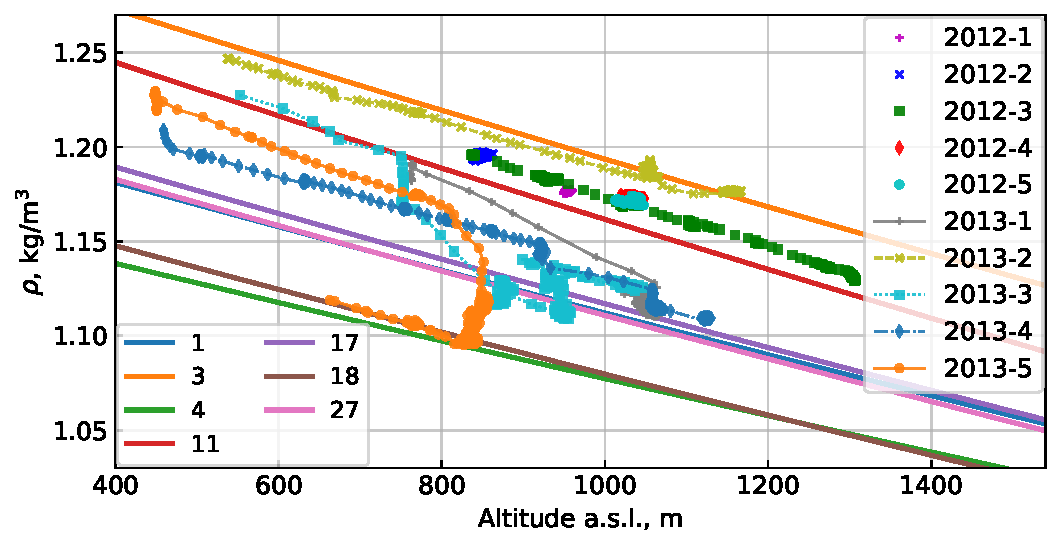
\includegraphics[width=15pc]{fig17.pdf}%
    \vspace{-1.0pc}
    \caption{Mass overburden versus altitude experimental data (points) in each flight and CORSIKA profiles (solid lines with corresponding models numbers).}
    \todoi{Картинка с измерениями (tele pic. 17)}
    \label{fig:fig17}
  \end{minipage}
\hfill
  \begin{minipage}[t]{0.48\textwidth}
    \centering
    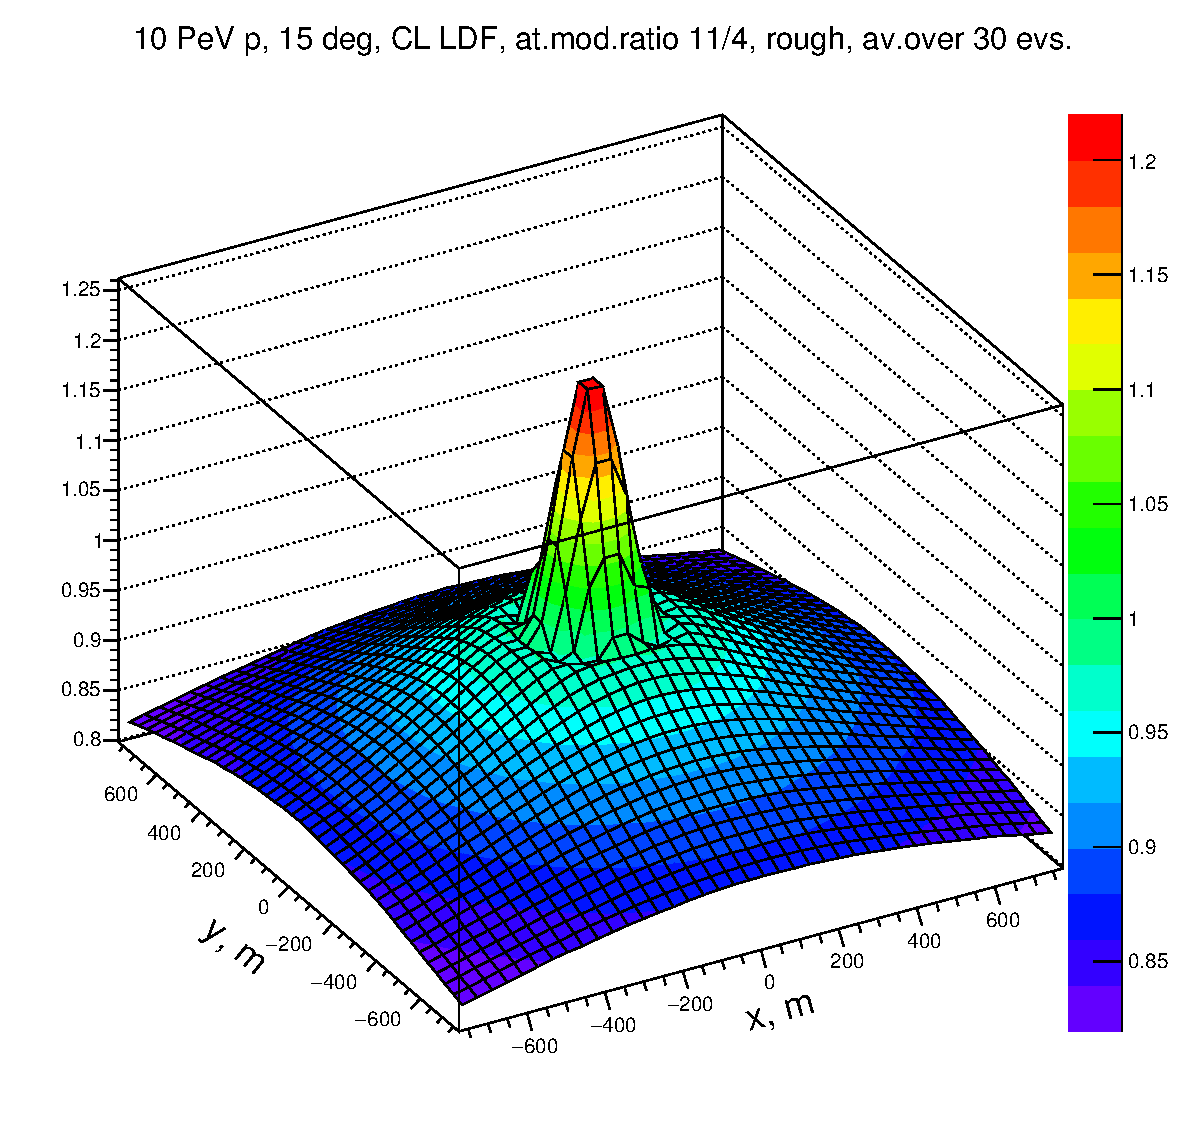
\includegraphics[width=15pc]{11d4}%
    \vspace{-1.0pc}
    \caption{Sample mean Cherenkov light lateral distribution ratio for CORSIKA atmosphere model
    pair 11/4. Bin size 50~m $\times$ 50~m. 10~PeV primary protons. Zenith angle 15~$\deg$. Sample volume 30~events.}
    \todoi{Картинка с ФПР ЧС при нескольких разных атмосферах из набора подходящих к точкам (tele pic. 20-21)}
\label{fig:4d11}
\end{minipage}
\end{figure}


% * Написать про важность контроля -- ссылки на работы про это поискать. 
% * Уникальная возможность измерять состояние нижнего слоя атмосферы прямо на самой установке.
% * Возможность использования вспомогательных дронов

\subsection{Surface properties}

\todoi{Описание работы с ровным/неровным снегом, проверка отражающей способности, чем можно. (Чернов)}

\section{Analysis methods}
\subsection{CL LDF reconstruction}
\todoi{Деконволюция, режим сканирования (Подгрудков, Вайман)}

\subsection{Axis, angles, energy}
\todoi{Определение сигнала, оси и пр. (Подгрудков, Вайман)}
\subsection{Primary type}
\todoi{Методика разделения типов первичных частиц (Латыпова, Галкин).}

%Modeling procedure generally follows the approach used in SPHERE-2 experiment. It includes event modeling and image processing.
%Event modeling incorporates two stages: a) EAS simulation with CORSIKA code including Cherenkov light generation and b) the production of CL images of EAS events in the telescope mosaic. The 1st stage results in a detailed 3D-array of CL photoelecton distribution in coordinates and time delay on the snow for each EAS event. Photoelectons appear due to a special CORSIKA mode enabling account for the PMT efficiency during the shower modeling. At the 2nd stage the shower cores on the snow are evenly spread over a circle of 500 m radius centered under the telescope. Contributions to the mosaic PMTs from every patch of the CL spot on the snow are calculated on photoelectron-by-photoelectron basis.

Primary mass estimation method uses the shape of an EAS CL image in the telescope mosaic. Firstly, the images are fitted with an axisymmetric rational function. Secondly, the approximations are integrated over a central circle and the surrounding ring. Thirdly, a ratio of these integrals is used as a criterion parameter for the separation of events by the primary mass. Criteria are optimized with respect to the mass separation by varying the radii of the circle and the ring. Optimal criteria are obtained for different primary energies and zenith angles, detector elevation and atmosphere models (1 and 11 in CORSIKA terms).

One can rely on the primary energy and zenith angle estimates derived from the event data and thus use different criteria for different combinations of these primary parameters and also for different values of the detector elevation which is measurable. Atmosphere model affects the mass criteria as well and must be taken into account while processing the images.
We hope to be able to promptly register the parameters of the local atmosphere (up to at least 20 km above the snow) during the experiment. Hadron interaction at super high energies presents another problem as its different models lead to different shower behaviours. According to our experience, the use of shape characteristics as criterion parameter substantially reduces the effect of interaction model on primary mass criterion. Still, the effect must be known and the final criterion should be selected in such a way so as to minimize its dependence on the model.

One more possibility to improve the primary mass resolution is the use of the direct CL angular distribution which is proved to be a powerful instrument for this task\cite{Gal18a}.

\todoi{Про оптимизацию геометрии и критерия друг под друга. (Галкин)}
The design of the telescope and the circumstances of the experiment (such as detector elevation height) affect the mass separation procedure and the resulting primary mass resolution. As we aim at constructing a detector for the solution of the primary cosmic ray mass composition problem we have to optimize the detector design with respect to this goal. To do so we are sentenced to consider a few experiment configurations with the corresponding image processing techniques and choose the one with the best mass resolution.


\section{Discussion}
\todoi{Pro et con (all)}

\section{Conclusions}
\todoi{Выводы.}

\acknowledgments
\todoi{Гранты? (Чернов)}
M. Finger and M. Finger Jr thank MEYS of Czech Republic for grants LG14004 and LG18022.

\bibliographystyle{JHEP}
\bibliography{references}
\todoi{Ссылки. (Бонвеч)}

\end{document}
